\documentclass[12pt,a4paper]{article}
\usepackage[utf8]{inputenc}
\usepackage[T1]{fontenc}
\usepackage{lmodern}
\usepackage[english]{babel}
\usepackage{geometry}
\geometry{a4paper, margin=2.5cm}
\usepackage{graphicx}
\usepackage{longtable}
\usepackage{hyperref}
\usepackage{array}
\usepackage{amsmath}
\usepackage{amssymb}
\usepackage{enumitem}
\usepackage{tabularx}
\usepackage{tikz}
\usetikzlibrary{fit, positioning, calc, arrows.meta, shapes.geometric}
\usepackage{pgfgantt}
\usepackage{microtype}
\usepackage{booktabs}
\usepackage{listings}
\usepackage[style=ieee,backend=biber,doi=true,url=true]{biblatex}
\addbibresource{references.bib}

\hypersetup{
    colorlinks=true,
    linkcolor=blue,
    filecolor=magenta,      
    urlcolor=cyan,
    citecolor=blue,
    pdftitle={Edge-Cloud Collaborative Smart Surveillance System},
    pdfpagemode=FullScreen,
}

\begin{document}
\hypersetup{pageanchor=false}

% =========================================================================
% TRANG BÌA (TITLE PAGE)
% =========================================================================
\begin{titlepage}
    \begin{tikzpicture}[remember picture, overlay]
        \draw[line width = 3pt]
            ([shift={(1.5cm,-1.5cm)}]current page.north west)
            rectangle
            ([shift={(-1.5cm,1.5cm)}]current page.south east);
        \draw[line width = 1pt, double, double distance = 3pt]
            ([shift={(1.65cm,-1.65cm)}]current page.north west)
            rectangle
            ([shift={(-1.65cm,1.65cm)}]current page.south east);
    \end{tikzpicture}
    
    \begin{center}
        \textbf{\large MINISTRY OF EDUCATION AND TRAINING} \\
        \vspace{0.2cm}
        \textbf{\large FPT UNIVERSITY} \\
        \textbf{-------------------} \\
        \vspace{1.5cm}

        \begin{figure}[h]
            \centering
            % Dưới đây là ví dụ chèn hình ảnh logo trường FPT, có thể thay đổi bằng file logo thực tế
            % 
\includegraphics[width=0.4\textwidth]{Logo_Trường_Đại_học_FPT.png}
            
\begin{tikzpicture}
                \draw[fill=orange!10, orange, thick] (0,0) rectangle (4,1.5);
                \node at (2,0.75) {\textbf{\Large FPT UNIVERSITY}};
            \end{tikzpicture}
        \end{figure}
        \vspace{1.5cm}
        
        \textbf{\Large MASTER OF SOFTWARE ENGINEERING (MSE)} \\
        \vspace{0.5cm}
        \textbf{\Large GRADUATE THESIS PROPOSAL} \\
        \vspace{1.5cm}

        \begin{flushleft}
            \textbf{\Large Thesis Title:} \\
            \vspace{0.4cm}
            \textbf{\huge AN EDGE-CLOUD COLLABORATIVE IoT FRAMEWORK} \\
            \vspace{0.2cm}
            \textbf{\huge FOR REAL-TIME SMART SURVEILLANCE} \\
            \vspace{0.2cm}
            \textbf{\Large Integrating Dynamic Projection People Counting, Cosine Face Identification, and Multi-Hazard Anomaly Detection} \\
        \end{flushleft}
        
        \vspace{2cm}
        \begin{table}[h]
            \flushright
            \begin{tabular}{ll}
                \textbf{Academic Supervisor:} & \textbf{Dr. Doan Xuan Huy Minh} \\
                \textbf{Graduate Student:} & \textbf{Nguyen Van Toan} \\
                \textbf{Student ID / Class:} & \textbf{MSE26HCM} \\
            \end{tabular}
        \end{table}
        
        \vfill
        \textbf{Ho Chi Minh City, May 2026}
    \end{center}
\end{titlepage}
\hypersetup{pageanchor=true}

\newpage

% =========================================================================
% TÓM TẮT ĐỀ TÀI (ABSTRACT)
% =========================================================================
\section*{Abstract}
\addcontentsline{toc}{section}{Abstract}
In contemporary security management, the demand for smart, real-time, and privacy-preserving surveillance systems has grown exponentially. Commercial off-the-shelf cameras often rely heavily on cloud-based computation, introducing significant network latency, bandwidth overheads, and severe data privacy concerns. This capstone project proposal presents a comprehensive, lightweight, and low-cost IoT-Edge-Cloud collaborative framework designed for local real-time intelligent monitoring. 

The framework integrates four key functional capabilities deployed across an Edge layer and a Central Web Application: (1) an optimized multi-camera people counting model utilizing YOLOv8s and ByteTrack under a custom geometric double-line projection state machine with crossing cooldowns and dynamic state-inheritance; (2) a real-time face verification module leveraging Multitask Cascaded Convolutional Networks (MTCNN) for alignment, FaceNet for feature embedding generation, and cosine distance metric classification; (3) a Region-of-Interest (ROI) intrusion detection module utilizing YOLOv5; and (4) an automated fall detection system utilizing custom trained YOLOv8-fall weights. 

To prevent network blocking and streaming lag under real-time alerts, we implement an asynchronous multi-threaded notification dispatcher connecting directly to Telegram services. Preliminary experiments show that the system achieves high accuracy in crowd tracking, eliminates counting jitter near boundaries, and operates at $\ge$ 20 FPS on a CUDA-accelerated edge GPU with latency below 1.5 seconds. This proposed system establishes a robust, highly extensible architecture suitable for household and office automation.

\newpage

% =========================================================================
% MỤC LỤC
% =========================================================================
\tableofcontents
\newpage

% =========================================================================
% DANH MỤC TỪ VIẾT TẮT
% =========================================================================
\section*{List of Abbreviations}
\addcontentsline{toc}{section}{List of Abbreviations}

\begin{longtable}{ll}
\toprule
\textbf{Abbreviation} & \textbf{Definition} \\
\midrule
\endhead
\textbf{AI} & Artificial Intelligence \\
\textbf{API} & Application Programming Interface \\
\textbf{FPS} & Frames Per Second \\
\textbf{GPU} & Graphics Processing Unit \\
\textbf{HTTP} & Hypertext Transfer Protocol \\
\textbf{IoT} & Internet of Things \\
\textbf{mAP} & Mean Average Precision \\
\textbf{MSE} & Master of Software Engineering \\
\textbf{MTCNN} & Multitask Cascaded Convolutional Networks \\
\textbf{ROI} & Region of Interest \\
\textbf{UI/UX} & User Interface / User Experience \\
\textbf{VCF} & Variant Call Format \\
\textbf{YOLO} & You Only Look Once \\
\bottomrule
\end{longtable}

\newpage

% =========================================================================
% CHAPTER 1: INTRODUCTION
% =========================================================================
\section{Introduction}

\subsection{Background and Motivation}
In the contemporary landscape of smart buildings and home automation, security monitoring is a high-priority requirement. Traditional video surveillance systems primarily function as passive recording devices. The burden of identifying threats, tracking occupancy, and recognizing anomalies falls entirely on human operators, which is error-prone and labor-intensive. 

Recent advancements in Artificial Intelligence (AI) and Computer Vision (CV), particularly the development of high-performance object detection networks such as You Only Look Once (YOLO) and face recognition architectures like FaceNet, have opened the possibility of automated real-time monitoring. However, deploying such resource-intensive deep learning models in residential or small office environments introduces significant architectural challenges. 

A traditional cloud-only approach, where raw video feeds from multiple high-definition cameras are streamed continuously to remote cloud instances for analysis, is highly suboptimal. It suffers from high network latency, severe bandwidth utilization, and high operating costs. More importantly, uploading private indoor video streams to third-party servers raises significant data privacy and security concerns. 

To resolve these limitations, this thesis proposes a lightweight, localized \textbf{Edge-Cloud Collaborative IoT Framework} designed for smart surveillance. By deploying containerized AI pipelines on local edge processor nodes, the system processes video frames directly at the data source. Bandwidth consumption is minimized, latency is reduced to sub-second levels, and video data remains secure within the local network. The cloud/central console is utilized exclusively for metadata logging, system configuration updates, and alert notifications.

\subsection{Problem Statement}
Despite the promise of Edge-based AI video analytics, existing systems face several critical technical limitations:
\begin{enumerate}
    \item \textbf{Spatial Counting Inaccuracies near Boundaries (Jitter \& ID Swaps):} Standard people counting systems rely on a single virtual line. When individuals stand near the line, hesitate, or move back and forth, the system triggers duplicate counts. Furthermore, in crowded conditions, occlusion often causes the Multi-Object Tracking (MOT) engine to swap or drop tracking IDs, leading to state loss.
    \item \textbf{Visual Anomaly Recognition Failures under Pose/View Variation:} Face verification systems deployed in real-world scenarios must recognize individuals at non-frontal angles. Standard face identification models fail when subjects look sideways or tilt their heads. In addition, residential care requires the integration of diverse anomaly detectors (e.g., fall detection, intrusion, fire hazards) operating simultaneously without overloading the edge device.
    \item \textbf{Synchronous Thread Blocking during Alert Dispatches:} When an AI engine triggers an alert, it must transmit media capture data (images and videos) to supervisors. Performing synchronous HTTP post requests within the main camera frame capture loop introduces latency, leading to dropped frames, lag, and camera stream disconnections.
    \item \textbf{Tight Coupling and Poor Edge Resource Utilization:} Deploying multiple AI pipelines (YOLOv8, MTCNN, FaceNet, YOLOv5) concurrently on a consumer-grade CPU/GPU can lead to resource starvation, performance degradation, and system instability if the software architecture is not modularized and optimized.
\end{enumerate}

\subsection{Thesis Objectives}
To address these challenges, this capstone project realizes a fully integrated, edge-accelerated, and secure surveillance system. The specific technical objectives include:
\begin{itemize}
    \item \textbf{Objective 1:} Implement an optimized multi-camera tracking pipeline using YOLOv8s and ByteTrack, governed by a custom geometric double-line projection state machine with crossing cooldowns and track inheritance to eliminate boundary counting jitter.
    \item \textbf{Objective 2:} Design an aligned, multi-angle face verification module using MTCNN cascade tuning and FaceNet embeddings, achieving high accuracy for rotated/tilted faces.
    \item \textbf{Objective 3:} Deploy custom-trained YOLOv8-fall and fire anomaly detection models, managed within a circular buffer system to record and playback browser-compatible H.264 event videos.
    \item \textbf{Objective 4:} Develop an asynchronous, multi-threaded alert dispatcher and interactive two-way remote control using Telegram Long Polling, maintaining stable camera frame rates ($\ge 20$ FPS).
    \item \textbf{Objective 5:} Build a responsive, glassmorphic monitoring dashboard utilizing FastAPI, implementing custom HMAC-SHA256 session management and hardware resource health monitoring.
\end{itemize}

\subsection{Project Scope}
\begin{itemize}
    \item \textbf{Inclusions:} Real-time multi-camera frame capture and analysis; edge-accelerated object tracking and counting; local face registration and multi-view verification; Region-of-Interest (ROI) intrusion detection; pose/bounding-box-based fall detection; fire anomaly monitoring; localized H.264 video buffering; and secure, web-based settings management.
    \item \textbf{Exclusions:} Outdoor environmental modeling; integration with proprietary smart home systems (e.g., Apple HomeKit, Google Home); emotion recognition; and large-scale cloud database clustering.
\end{itemize}

\subsection{Organization of the Thesis}
The remainder of this thesis is structured as follows:
\begin{itemize}
    \item \textbf{Chapter 2 (Literature Review):} Evaluates existing architectures in Edge-Cloud IoT surveillance, tracking frameworks, facial verification techniques, and vision-based anomaly detection models.
    \item \textbf{Chapter 3 (Design and Implementation):} Details the system architecture, mathematical formulations, software components, and implementation specifics of the proposed framework.
    \item \textbf{Chapter 4 (Evaluation and Discussion):} Presents the experimental setup, quantitative results, and comparative benchmarks.
    \item \textbf{Chapter 5 (Conclusion and Future Work):} Summarizes the contributions and suggests future research directions.
\end{itemize}

\newpage

% =========================================================================
% CHAPTER 2: LITERATURE REVIEW
% =========================================================================
\section{Literature Review}

\subsection{Edge-Cloud IoT Frameworks in Video Surveillance}
Traditional video surveillance relies on central cloud computing where full high-definition video data is streamed continuously to remote cloud servers. Shi et al. \cite{shi_edge_2016} show that this approach is inefficient for real-time applications due to network congestion and latency. Gupta et al. \cite{gupta_ifogsim_2017} and Chen et al. \cite{chen_edge_2019} propose Edge-computing architectures, shifting intensive visual inference to local edge processor nodes. By processing video frames at the edge and transmitting only lightweight metadata (logs, alert flags, and brief image/video snapshots) to the central server, edge computing reduces network bandwidth consumption by up to 90\% and preserves data privacy.

\subsection{Object Detection and Multi-Object Tracking (MOT)}
Real-time object detection has been dominated by the You Only Look Once (YOLO) family. YOLOv8 \cite{yolov8_2023} provides an anchor-free detection format that outperforms previous versions in both accuracy and inference speed. In multi-camera counting environments, object detection must be paired with Multi-Object Tracking (MOT). ByteTrack \cite{bytetrack_2022} provides a robust association method by utilizing low-confidence detection boxes (often caused by occlusion or motion blur) instead of discarding them, maintaining track continuity during person-to-person overlaps.

\subsection{Face Verification and Embedding Extraction}
Face identification in unconstrained environments requires accurate detection, alignment, and representation. MTCNN \cite{mtcnn_2016} utilizes a three-stage cascade structure (P-Net, R-Net, O-Net) to detect face coordinates and facial landmarks (eyes, nose, mouth corners) even under head rotations. FaceNet \cite{facenet_2015} maps facial crops to a compact 128-dimensional Euclidean space where distances correspond directly to facial similarity, enabling verification and classification via thresholding.

\subsection{Visual Anomaly Detection: Fall and Fire Hazards}
Vision-based fall detection generally employs deep learning classifiers or pose estimation algorithms. While pose estimation models (e.g., YOLOv8-pose) provide keypoint joint coordinates, they are computationally expensive for resource-constrained edge devices. Custom-trained bounding box detectors (e.g., YOLOv8-fall) offer a lightweight alternative, identifying "fall" states based on bounding box aspect ratios and motion trajectories. Fire and smoke anomaly detection similarly utilizes YOLO-based networks, allowing edge nodes to process hazards concurrently alongside security tasks.

\subsection{State Machines in Spatial Crossing Analysis}
Single-line crossing models are highly sensitive to boundary jitter. When a tracked target hovers near the line, minor bounding box fluctuations cause duplicate counts. Implementing a parallel double-line crossing buffer zone, governed by a finite state machine, mitigates this issue. This transition zone acts as a hysteresis buffer, ensuring a count is registered only when the target completes a full transition from one side to the other.

\newpage

% =========================================================================
% CHAPTER 3: DESIGN AND IMPLEMENTATION
% =========================================================================
\section{Design and Implementation}

\subsection{Overall System Architecture and Data Flow}
The proposed framework is designed as an Edge-Cloud Collaborative IoT architecture. The system is split into two primary layers:
\begin{enumerate}
    \item \textbf{Edge Processing Layer:} Deployed on the local hardware node, this layer handles real-time video capture, frames preprocessing, deep learning inference (YOLOv8s object tracking, MTCNN facial detection, FaceNet embedding extraction, and anomaly detection), and state tracking. It manages a circular frame buffer for video event recording.
    \item \textbf{Backend \& Core Web Dashboard Layer:} Implemented using FastAPI (Python), this layer exposes web interfaces, manages the database (SQLite \texttt{faces.db}), and coordinates settings. An asynchronous dispatcher handles notifications.
\end{enumerate}

\begin{figure}[htbp]
    \centering
    \resizebox{\textwidth}{!}{%
    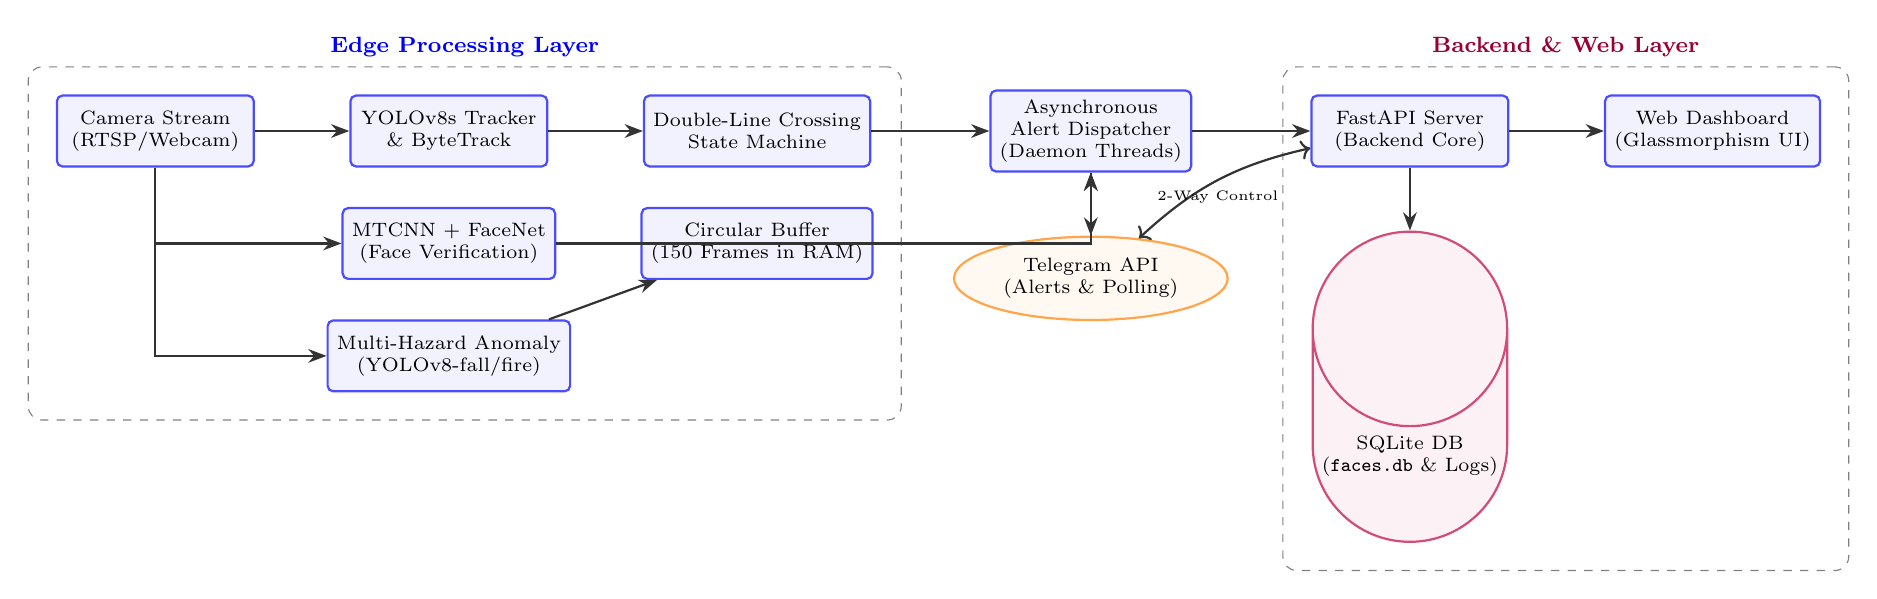
\begin{tikzpicture}[
        node distance=1.2cm and 1.5cm,
        box/.style={rectangle, draw=blue!70, fill=blue!5, thick, minimum width=2.5cm, minimum height=0.9cm, align=center, rounded corners=2pt, font=\scriptsize},
        database/.style={cylinder, draw=purple!70, fill=purple!5, thick, minimum width=1.6cm, minimum height=1.1cm, shape border rotate=90, align=center, font=\scriptsize},
        cloud_node/.style={ellipse, draw=orange!70, fill=orange!5, thick, minimum width=2.4cm, minimum height=0.9cm, align=center, font=\scriptsize},
        arrow/.style={-Stealth, thick, draw=black!80},
        container/.style={draw=gray, dashed, inner sep=0.35cm, rounded corners=5pt}
    ]
        % --- EDGE LAYER ---
        \node[box] (camera) {Camera Stream\\(RTSP/Webcam)};
        \node[box, right=1.2cm of camera] (yolo) {YOLOv8s Tracker\\\& ByteTrack};
        \node[box, below=0.5cm of yolo] (facenet) {MTCNN + FaceNet\\(Face Verification)};
        \node[box, below=0.5cm of facenet] (anomaly) {Multi-Hazard Anomaly\\(YOLOv8-fall/fire)};
        
        \node[box, right=1.2cm of yolo] (doubleline) {Double-Line Crossing\\State Machine};
        \node[box, below=0.5cm of doubleline] (buffer) {Circular Buffer\\(150 Frames in RAM)};
        
        % --- CONNECTIONS IN EDGE ---
        \draw[arrow] (camera) -- (yolo);
        \draw[arrow] (camera) |- (facenet);
        \draw[arrow] (camera) |- (anomaly);
        
        \draw[arrow] (yolo) -- (doubleline);
        \draw[arrow] (anomaly) -- (buffer);
        
        % Edge Border
        \node[container, fit=(camera) (yolo) (anomaly) (doubleline) (buffer), label={[font=\footnotesize, text=blue]\textbf{Edge Processing Layer}}] (edge_group) {};
        
        % --- DISPATCHER & CLOUD/BACKEND ---
        \node[box, right=1.5cm of doubleline] (dispatcher) {Asynchronous\\Alert Dispatcher\\(Daemon Threads)};
        \node[cloud_node, below=0.8cm of dispatcher] (telegram) {Telegram API\\(Alerts \& Polling)};
        
        % --- BACKEND / WEB DASHBOARD LAYER ---
        \node[box, right=1.5cm of dispatcher] (fastapi) {FastAPI Server\\(Backend Core)};
        \node[database, below=0.8cm of fastapi] (db) {SQLite DB\\(\texttt{faces.db} \& Logs)};
        \node[box, right=1.2cm of fastapi] (dashboard) {Web Dashboard\\(Glassmorphism UI)};
        
        % --- CONTAINER FOR BACKEND ---
        \node[container, fit=(fastapi) (db) (dashboard), label={[font=\footnotesize, text=purple!80!black]\textbf{Backend \& Web Layer}}] (backend_group) {};
        
        % --- CROSS-LAYER CONNECTIONS ---
        \draw[arrow] (doubleline) -- (dispatcher);
        \draw[arrow] (buffer) -| (dispatcher);
        \draw[arrow] (facenet) -| (dispatcher);
        
        \draw[arrow] (dispatcher) -- (telegram);
        \draw[arrow] (dispatcher) -- (fastapi);
        
        \draw[arrow] (fastapi) -- (db);
        \draw[arrow] (fastapi) -- (dashboard);
        \draw[arrow, <->, bend left=15] (telegram) to node[midway, below, font=\tiny] {2-Way Control} (fastapi);
        
    \end{tikzpicture}%
    }
    \caption{Detailed System Architecture Data Flow}
    \label{fig:detailed_architecture}
\end{figure}

\subsection{Projection-based Double-Line Crossing Model}
To resolve boundary jitter and false directional counts, we present a mathematical model of our custom projection double-line crossing algorithm.

Let a user-drawn counting line segment be defined by endpoints $A(x_1, y_1)$ and $B(x_2, y_2)$. The directional line segment vector is:
\begin{equation}
    \mathbf{v}_{line} = B - A = (x_2 - x_1, y_2 - y_1)
\end{equation}
The length of the baseline is $L = \|\mathbf{v}_{line}\|_2 = \sqrt{(x_2 - x_1)^2 + (y_2 - y_1)^2}$.
We define the perpendicular unit normal vector $\mathbf{n} = (n_x, n_y)$ as:
\begin{equation}
    n_x = -\frac{y_2 - y_1}{L}, \quad n_y = \frac{x_2 - x_1}{L}
\end{equation}
The normal vector points towards the direction of entry (defined via \texttt{in\_direction}). We establish a parallel double-line crossing buffer zone of width $2d$ (where $d = 30$ pixels) along the normal axis. The two virtual boundaries, the \textbf{Outer Line} and the \textbf{Inner Line}, are positioned at offsets of $-d$ and $+d$, respectively.

For any tracked pedestrian ID $tid$ at frame $t$, let their bottom-center bounding box coordinate be $P = (x_{bc}, y_{bc})$. The scalar projection distance $v(P)$ of the person relative to the baseline along the normal vector is computed as:
\begin{equation}
    v(P) = (x_{bc} - x_1) n_x + (y_{bc} - y_1) n_y
\end{equation}
Using the value of $v(P)$, the position is classified into one of three discrete regions $R(P) \in \{1, 2, 3\}$:
\begin{equation}
    R(P) = \begin{cases} 
      1 \quad \text{(Region 1 - Outside)}, & v(P) < -d \\
      2 \quad \text{(Region 2 - Transition Zone)}, & -d \le v(P) \le d \\
      3 \quad \text{(Region 3 - Inside)}, & v(P) > d 
   \end{cases}
\end{equation}

Depending on the configuration, Region 1 is mapped to \texttt{outside\_reg} and Region 3 is mapped to \texttt{inside\_reg}. The system maintains a state vector for each active tracker ID:
\begin{equation}
    S(\text{tid}) = (s_{\text{state}},\, t_{\text{last\_cross}})
\end{equation}
where $s_{\text{state}} \in \{\text{from\_outside},\, \text{from\_inside}\}$ represents the starting boundary, and $t_{\text{last\_cross}}$ is the frame index of the most recent crossing event.

\subsubsection{State Transitions and Cooldown Filtering}
State updates and count increments occur according to the following state machine:
\begin{itemize}
    \item \textbf{Case A:} The pedestrian is detected in the outside region ($R(P) = \text{outside\_reg}$):
    \begin{equation}
        S(\text{tid}) \leftarrow \begin{cases} 
          (\text{from\_outside},\, t_{\text{curr}}), & \text{if } s_{\text{state}} = \text{from\_inside} \text{ and } t_{\text{curr}} - t_{\text{last\_cross}} > \theta_{\text{cooldown}} \\
          (s_{\text{state}},\, t_{\text{last\_cross}}), & \text{otherwise}
       \end{cases}
    \end{equation}
    If the update is triggered, the local counter increments the \textbf{OUT} count by 1. Here, the refractory cooldown period is set to $\theta_{\text{cooldown}} = 45$ frames.
    
    \item \textbf{Case B:} The pedestrian is detected in the inside region ($R(P) = \text{inside\_reg}$):
    \begin{equation}
        S(\text{tid}) \leftarrow \begin{cases} 
          (\text{from\_inside},\, t_{\text{curr}}), & \text{if } s_{\text{state}} = \text{from\_outside} \text{ and } t_{\text{curr}} - t_{\text{last\_cross}} > \theta_{\text{cooldown}} \\
          (s_{\text{state}},\, t_{\text{last\_cross}}), & \text{otherwise}
       \end{cases}
    \end{equation}
    If the update is triggered, the local counter increments the \textbf{IN} count by 1.
\end{itemize}

\begin{figure}[htbp]
    \centering
    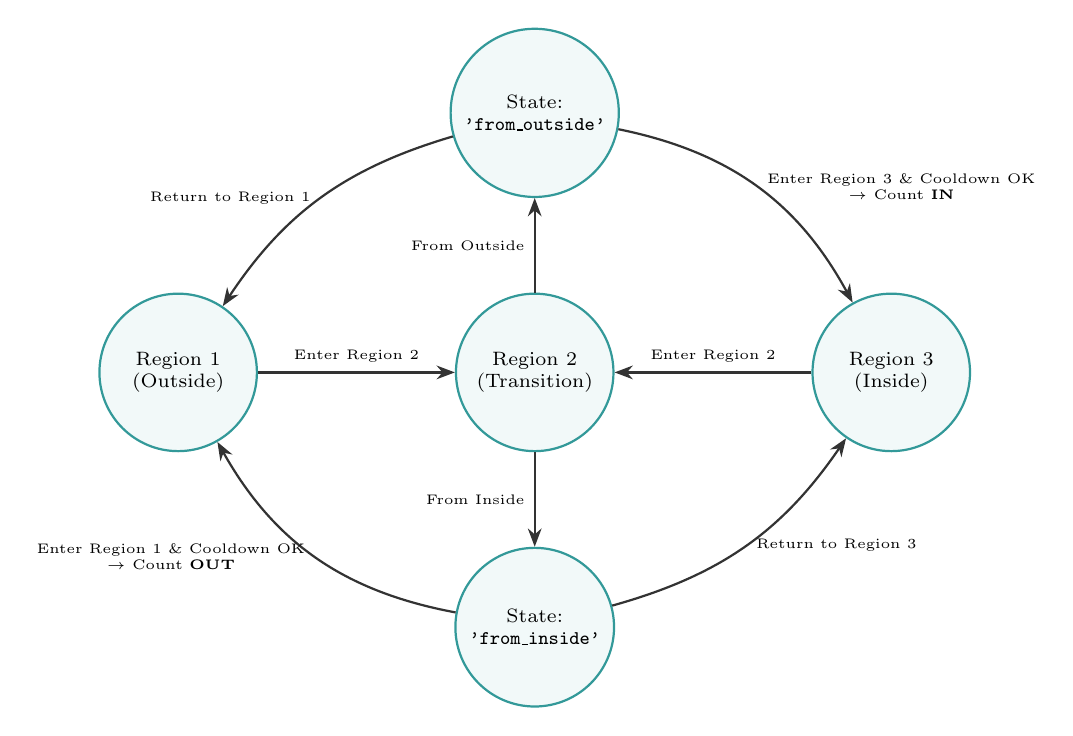
\begin{tikzpicture}[
        node distance=2.2cm and 2.5cm,
        state/.style={circle, draw=teal!80, fill=teal!5, thick, minimum size=2.0cm, align=center, font=\scriptsize},
        transition/.style={rectangle, draw=gray, fill=gray!5, dashed, minimum size=1.5cm, align=center, font=\scriptsize},
        arrow/.style={-Stealth, thick, draw=black!80}
    ]
        % --- NODES ---
        \node[state] (outside) {Region 1\\(Outside)};
        \node[state, right=of outside] (transition) {Region 2\\(Transition)};
        \node[state, right=of transition] (inside) {Region 3\\(Inside)};
        
        % --- TRANSITION SUBSTATES ---
        \node[state, above=1.2cm of transition] (from_outside) {State:\\\texttt{'from\_outside'}};
        \node[state, below=1.2cm of transition] (from_inside) {State:\\\texttt{'from\_inside'}};
        
        % --- ARROWS ---
        % Outside to transition
        \draw[arrow] (outside) -- (transition) node[midway, above, font=\tiny] {Enter Region 2};
        \draw[arrow] (inside) -- (transition) node[midway, above, font=\tiny] {Enter Region 2};
        
        % Transition to states
        \draw[arrow] (transition) -- (from_outside) node[midway, left, font=\tiny] {From Outside};
        \draw[arrow] (transition) -- (from_inside) node[midway, left, font=\tiny] {From Inside};
        
        % Completing crossing
        \draw[arrow, bend left=25] (from_outside) to node[midway, right, font=\tiny, align=center] {Enter Region 3 \& Cooldown OK\\$\rightarrow$ Count \textbf{IN}} (inside);
        \draw[arrow, bend left=25] (from_inside) to node[midway, left, font=\tiny, align=center] {Enter Region 1 \& Cooldown OK\\$\rightarrow$ Count \textbf{OUT}} (outside);
        
        % Aborted crossings
        \draw[arrow, bend right=20] (from_outside) to node[midway, left, font=\tiny] {Return to Region 1} (outside);
        \draw[arrow, bend right=20] (from_inside) to node[midway, right, font=\tiny] {Return to Region 3} (inside);
        
    \end{tikzpicture}
    \caption{Finite State Machine (FSM) for Parallel Double-Line Crossing}
    \label{fig:crossing_fsm}
\end{figure}

\subsection{Dynamic Lost-Track State Inheritance}
When pedestrians overlap, or are temporarily occluded by visual obstacles, the MOT engine can drop their detection box, clearing their state from memory. Upon recovery, they are assigned a new tracker ID. To avoid counting losses, we propose a \textbf{Dynamic Lost-Track Inheritance} heuristic.

When an active ID $tid_{\text{lost}}$ is lost, its state tuple $S(tid_{\text{lost}})$ and its final position $P_{\text{last}}$ are stored in a buffer $H_{\text{lost}}$ for up to 150 frames. When a new tracker ID $tid_{\text{new}}$ appears at frame $t_{\text{curr}}$ with coordinate $P_{\text{new}}$:
We calculate the Euclidean distance $D = \|P_{\text{new}} - P_{\text{last}}\|_2$ for all candidates in $H_{\text{lost}}$. An inheritance match is established if:
\begin{equation}
    t_{\text{curr}} - t_{\text{lost}} < 150 \text{ frames} \quad \text{and} \quad D < \theta_{\text{threshold}}
\end{equation}
The distance threshold $\theta_{\text{threshold}}$ is dynamically bounded based on the object's scale and elapsed frames to model real-world movement limits:
\begin{equation}
    \theta_{\text{threshold}} = \min\left(150.0,\, 0.5 \times \max(W_{\text{bbox}}, H_{\text{bbox}}) + 3.5 \times (t_{\text{curr}} - t_{\text{lost}})\right)
\end{equation}
Upon finding the minimum distance candidate satisfying these bounds, $tid_{\text{new}}$ inherits the historical state tuple $S(tid_{\text{lost}})$, preserving the crossing state machine.

\begin{lstlisting}[language=Python, caption={Dynamic Lost-Track State Inheritance Algorithm}, label={alg:track_inheritance}, frame=single, basicstyle=\ttfamily\scriptsize]
Algorithm 1: Dynamic Lost-Track State Inheritance
Input: 
  new_tracks: List of newly detected active tracker objects in frame t
  lost_buffer: Queue of historically lost tracker states H_lost up to 150 frames
  lost_track_window: 150 frames
  dist_threshold_max: 150.0 pixels

for new_tr in new_tracks:
    curr_pos = new_tr.bottom_center_coordinate
    bbox_dim = max(new_tr.width, new_tr.height)
    
    best_match_tid = None
    best_match_dist = infinity
    
    for lost_tid, (lost_state_tuple, lost_pos, lost_frame) in lost_buffer.items():
        elapsed_frames = t - lost_frame
        
        if elapsed_frames < lost_track_window:
            dist = EuclideanDistance(curr_pos, lost_pos)
            
            # Dynamically compute search threshold bounding speed
            max_allowed_dist = min(dist_threshold_max, 
                                   0.5 * bbox_dim + 3.5 * elapsed_frames)
            
            if dist < max_allowed_dist and dist < best_match_dist:
                best_match_tid = lost_tid
                best_match_dist = dist
                
    if best_match_tid is not None:
        # Match found: inherit historical state
        new_tr.state_tuple = lost_buffer[best_match_tid].state_tuple
        remove best_match_tid from lost_buffer
    else:
        # No match found: initialize new state
        new_tr.state_tuple = None
\end{lstlisting}

\subsubsection{Novelty Validation Case Study}
To demonstrate the mathematical validity and practical novelty of the proposed lost-track state inheritance model, we evaluate the system behavior under two distinct scenarios during a person-to-person occlusion event:
\begin{itemize}
    \item \textbf{Scenario A (Baseline Multi-Object Tracking):} An individual tracked as ID 15 approaches the virtual counting baseline. During a brief overlap with another pedestrian, the bounding box is obscured, causing the ByteTrack engine to drop the track ID. Upon emerging 10 frames later, the tracker assigns a new ID 26 to the same pedestrian. Because ID 26 has no prior history, its transition through the FSM triggers a duplicate crossing count, yielding a false positive error.
    \item \textbf{Scenario B (Proposed Framework):} When ID 15 is dropped, its final position $P_{\text{last}}$ and state tuple $S(\text{ID } 15)$ are buffered in $H_{\text{lost}}$. When the person emerges and is assigned ID 26, the inheritance engine checks $H_{\text{lost}}$. Since the spatial distance $D$ satisfies $D < \theta_{\text{threshold}}$ and the temporal gap is only 10 frames, ID 26 inherits $S(\text{ID } 15)$ (originally in state \texttt{'from\_outside'}). When ID 26 crosses the inner boundary, it completes the transition smoothly. The system registers a single correct count, successfully preserving track integrity.
\end{itemize}

\subsection{Face Recognition Pipeline with Profile/Tilted Adaptation}
Real-time facial verification is designed as a three-stage pipeline (Figure \ref{fig:face_pipeline}): detection, alignment and embedding extraction, and matching.

\begin{figure}[h]
    \centering
    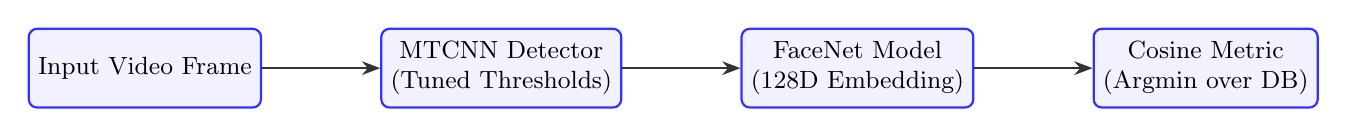
\begin{tikzpicture}[
        box/.style={rectangle, draw=blue!80, fill=blue!5, thick, minimum width=2.5cm, minimum height=1cm, align=center, rounded corners=3pt, font=\small},
        arrow/.style={-Stealth, thick, draw=black!80}
    ]
        \node[box] (input) {Input Video Frame};
        \node[box, right=1.5cm of input] (mtcnn) {MTCNN Detector\\(Tuned Thresholds)};
        \node[box, right=1.5cm of mtcnn] (facenet) {FaceNet Model\\(128D Embedding)};
        \node[box, right=1.5cm of facenet] (matching) {Cosine Metric\\(Argmin over DB)};
        
        \draw[arrow] (input) -- (mtcnn);
        \draw[arrow] (mtcnn) -- (facenet);
        \draw[arrow] (facenet) -- (matching);
    \end{tikzpicture}
    \caption{Three-Stage Facial Verification Pipeline}
    \label{fig:face_pipeline}
\end{figure}

To improve the detection rate of turned or tilted heads, the MTCNN cascade thresholds are tuned down to $\theta_{mtcnn} = [0.5, 0.6, 0.6]$ for P-Net, R-Net, and O-Net respectively. For face representation, FaceNet maps facial crops to 128-dimensional embeddings, which are $L_2$ normalized to unit length. 

We compare the real-time embedding vector $\mathbf{u}$ against all registered embeddings in the database. Let the registered embeddings for target $i$ be $\{\mathbf{v}_i^{(1)}, \mathbf{v}_i^{(2)}, \dots, \mathbf{v}_i^{(K)}\}$, representing different viewpoints (e.g., frontal, left-profile, right-profile, tilted-up, tilted-down). The matching distance is determined as the minimum cosine distance:
\begin{equation}
    d_{match} = \min_{j \in \{1,\dots,K\}} \left( 1 - \frac{\mathbf{u} \cdot \mathbf{v}_i^{(j)}}{\|\mathbf{u}\|_2 \|\mathbf{v}_i^{(j)}\|_2} \right)
\end{equation}
A subject is recognized if $d_{match} < \theta_{face}$, where $\theta_{face}$ is a configurable threshold (typically set between $0.65$ and $0.75$).

\subsection{Multi-Hazard Anomaly Detection and H.264 Video Buffering}
The anomaly detection subsystem operates three detection modules simultaneously:
\begin{itemize}
    \item \textbf{YOLOv5 ROI Intrusion Detector:} Evaluates if the bounding box center of a detected person falls within a polygon Region of Interest (ROI) defined dynamically in the configuration.
    \item \textbf{YOLOv8-fall Detection Model:} Custom-trained on the ImViA dataset (9.37GB containing Home, Office, Coffee room, and Lecture room clips). The training pipeline utilized 35,041 frames for training and 6,989 frames for validation, producing the weight file \texttt{yolov8n\_fall\_best.pt}.
    \item \textbf{YOLOv8n-fire Model:} Detects fire and smoke boundaries.
\end{itemize}

To provide contextual feedback during anomalies, each camera maintains a circular frame queue \texttt{state.frame\_buffer} in RAM holding the last 150 processed frames (approximately 10 seconds). When a hazard is detected, a worker thread is spawned to save the buffered frames as an H.264 encoded \texttt{.mp4} file.
We use the \texttt{avc1} codec first to ensure direct playback in web browsers. If the platform lacks the H.264 library, the module automatically falls back to \texttt{mp4v} to prevent system failure.
To prevent file-serving errors on Windows due to url-encoding of non-ASCII characters or spaces in camera names (e.g., "quet khuon mat"), all generated filenames are sanitized to ASCII alphanumeric formats using \texttt{sanitize\_filename\_component()}.

\subsection{Asynchronous Dispatcher and 2-way Telegram Remote Control}
Alerts are managed through an asynchronous thread dispatcher. When an event is triggered, the system clones the current frame, accesses the frame buffer, and dispatches the alert payload in a daemon background thread. This keeps the main camera capture thread free, maintaining stable frame rates.

We implement a two-way control loop using Telegram Long Polling. A worker thread runs a polling loop contacting the Telegram API. The bot registers callbacks from custom inline buttons attached to alert images (e.g., \texttt{Mute Alerts} or \texttt{Pause Cam 30m}). When clicked, the Telegram callback is received by the edge node, updating the FastAPI system settings dynamically.

\subsection{Web Dashboard \& Session Security}
The central dashboard is designed with a responsive Glassmorphism UI using HTML5, Vanilla CSS3, and Javascript. 
To secure the console without external dependencies, we implemented a custom \texttt{HMACSessionMiddleware}. It signs and verifies session cookies using HMAC-SHA256 with a local secret key. The dashboard includes a system health monitoring widget displaying real-time CPU and RAM usage, GPU load, VRAM allocation, and actual camera processing frame rates (FPS).

\subsection{Computational Complexity Analysis}
Deploying multiple deep learning and object tracking modules concurrently on an edge processor requires a clear understanding of the computational bounds. We present the asymptotic complexity of each core pipeline module in Table \ref{tab:complexity}.

\begin{table}[h]
    \centering
    \caption{Computational Complexity of Proposed System Modules}
    \label{tab:complexity}
    \begin{tabular}{lll}
        \toprule
        \textbf{Module} & \textbf{Time Complexity} & \textbf{Key Factor} \\
        \midrule
        YOLOv8s Object Detection & Proportional to $W \times H$ & Frame resolution width $W$ and height $H$ \\
        ByteTrack Association & $O(N \cdot M)$ & Detections $N$ and active tracks $M$ per frame \\
        Face Embeddings Matching & $O(K)$ & Total registered facial views $K$ in SQLite \\
        Lost-Track State Inheritance & $O(|H_{\text{lost}}|)$ & Size of lost tracks buffer $|H_{\text{lost}}| \le 10$ \\
        \bottomrule
    \end{tabular}
\end{table}

As shown in Table \ref{tab:complexity}, the processing time for the YOLOv8s object detector is directly proportional to the spatial resolution $W \times H$ of the input frames, representing the approximate computational complexity of CNN grid inference rather than a strict theoretical bounding box.

\subsection{Database Design and Relational Schema}
The localized storage subsystem uses SQLite to ensure zero-administration overhead on the edge node. The database file \texttt{faces.db} implements three main tables: \texttt{User}, \texttt{FaceRecord}, and \texttt{SystemEventLog}. The schema details are described below:

\begin{itemize}
    \item \textbf{Table \texttt{User}:} Stores administrator and operator login credentials.
    \begin{itemize}
        \item \texttt{id} (INTEGER, Primary Key, Auto-increment)
        \item \texttt{username} (VARCHAR, Unique, Not Null)
        \item \texttt{password\_hash} (VARCHAR, Not Null, PBKDF2 hash)
        \item \texttt{role} (VARCHAR, default \texttt{'admin'}, represents user access level: \texttt{'admin'} or \texttt{'operator'})
    \end{itemize}
    \item \textbf{Table \texttt{FaceRecord}:} Stores registered user facial identities and their corresponding FaceNet features.
    \begin{itemize}
        \item \texttt{id} (INTEGER, Primary Key, Auto-increment)
        \item \texttt{name} (VARCHAR, Not Null, name of the registered person)
        \item \texttt{embedding} (TEXT, Not Null, stores the 128D FaceNet embedding vector serialized as a JSON string)
        \item \texttt{created\_at} (VARCHAR, date of registration)
        \item \texttt{created\_by} (VARCHAR, name of the user who registered the face)
    \end{itemize}
    \item \textbf{Table \texttt{SystemEventLog}:} Records security logs including ROI intrusion alerts, fall detections, fire anomalies, and stranger face events.
    \begin{itemize}
        \item \texttt{id} (INTEGER, Primary Key, Auto-increment)
        \item \texttt{event\_type} (VARCHAR, e.g., \texttt{'intrusion'}, \texttt{'fall'}, \texttt{'fire'}, \texttt{'face'}, \texttt{'counter'})
        \item \texttt{message} (TEXT, Not Null, descriptive alert details)
        \item \texttt{camera\_id} (VARCHAR, Not Null)
        \item \texttt{image\_path} (VARCHAR, relative path to JPEG snapshot capture)
        \item \texttt{video\_path} (VARCHAR, relative path to H.264 event MP4 clip, Nullable)
        \item \texttt{face\_name} (VARCHAR, name of the recognized person, Nullable)
        \item \texttt{timestamp} (VARCHAR, default current timestamp formatted as \texttt{\%Y-\%m-\%d \%H:\%M:\%S})
    \end{itemize}
\end{itemize}

\begin{figure}[htbp]
    \centering
    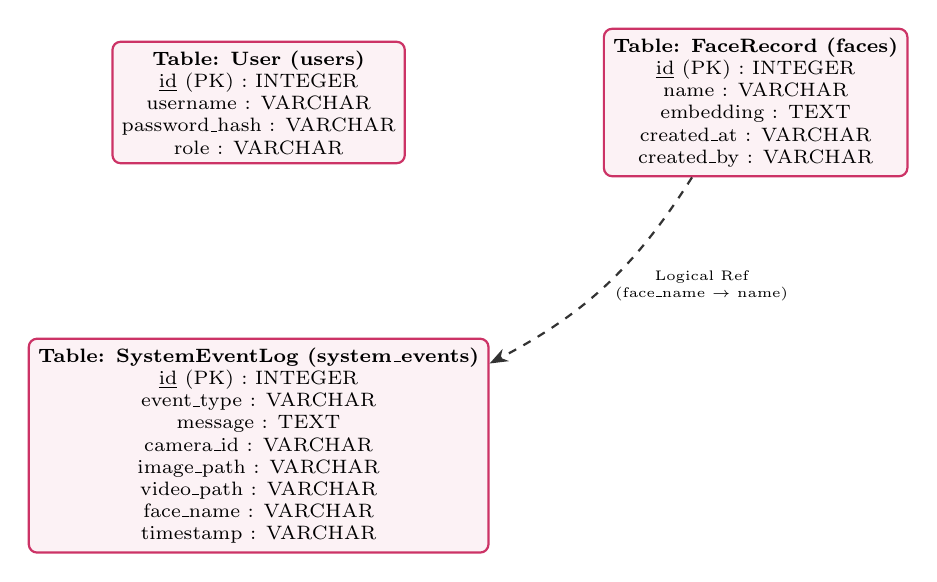
\begin{tikzpicture}[
        node distance=1.8cm and 2.5cm,
        entity/.style={rectangle, draw=purple!80, fill=purple!5, thick, minimum width=3.6cm, minimum height=1.3cm, align=center, rounded corners=3pt, font=\scriptsize},
        arrow/.style={-Stealth, thick, draw=black!80},
        cardinality/.style={font=\tiny, near start, above}
    ]
        \node[entity] (user) {\textbf{Table: User (users)} \\ \underline{id} (PK) : INTEGER \\ username : VARCHAR \\ password\_hash : VARCHAR \\ role : VARCHAR};
        
        \node[entity, right=of user] (faces) {\textbf{Table: FaceRecord (faces)} \\ \underline{id} (PK) : INTEGER \\ name : VARCHAR \\ embedding : TEXT \\ created\_at : VARCHAR \\ created\_by : VARCHAR};
        
        \node[entity, below=2.2cm of user] (eventlog) {\textbf{Table: SystemEventLog (system\_events)} \\ \underline{id} (PK) : INTEGER \\ event\_type : VARCHAR \\ message : TEXT \\ camera\_id : VARCHAR \\ image\_path : VARCHAR \\ video\_path : VARCHAR \\ face\_name : VARCHAR \\ timestamp : VARCHAR};
        
        \draw[arrow, dashed, bend left=15] (faces) to node[midway, right, font=\tiny, align=center] {Logical Ref\\(face\_name $\rightarrow$ name)} (eventlog);
    \end{tikzpicture}
    \caption{Database Entity-Relationship (ER) Diagram}
    \label{fig:database_erd}
\end{figure}

\subsection{Security and Privacy Considerations}
Security and user privacy are prioritized by design across all system layers:
\begin{itemize}
    \item \textbf{Biometric Privacy:} No raw facial photographs are stored in the database. During registration, the system extracts the 128D embedding and immediately discards the image. This prevents the reconstruction of user faces in the event of database leaks.
    \item \textbf{Session Security:} The custom \texttt{HMACSessionMiddleware} signs session cookies using HMAC-SHA256 with a locally rotated secret key. This prevents session tampering and credential hijacking without relying on third-party security libraries.
    \item \textbf{On-Premise Computation:} All visual processing and camera streams reside strictly within the local area network. No video files or streams are uploaded to external cloud instances, preserving local data sovereignty.
    \item \textbf{Telegram Authorization:} Telegram alert messages and inline button controls are restricted to authorized Chat IDs. The polling engine filters out unauthorized requests, securing remote commands.
\end{itemize}

\subsection{Use Case and Physical Deployment Modeling}
To define system boundaries, we present the Use Case Model in Figure \ref{fig:use_case} and the Hardware Deployment Diagram in Figure \ref{fig:deployment}.

\begin{figure}[htbp]
    \centering
    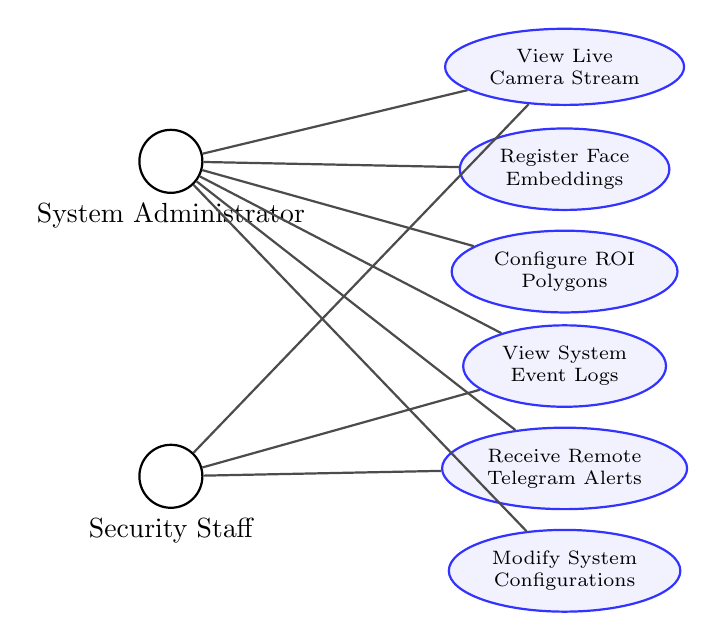
\begin{tikzpicture}[
        actor/.style={circle, draw=black, thick, minimum size=0.8cm, label=below:#1},
        usecase/.style={ellipse, draw=blue!80, fill=blue!5, thick, minimum width=2.4cm, minimum height=0.8cm, align=center, font=\scriptsize},
        arrow/.style={-, thick, draw=black!70}
    ]
        % --- ACTORS ---
        \node[actor={System Administrator}] (admin) at (0, 2) {};
        \node[actor={Security Staff}] (staff) at (0, -2) {};
        
        % --- USE CASES ---
        \node[usecase] (uc1) at (5, 3.2) {View Live\\Camera Stream};
        \node[usecase] (uc2) at (5, 1.9) {Register Face\\Embeddings};
        \node[usecase] (uc3) at (5, 0.6) {Configure ROI\\Polygons};
        
        \node[usecase] (uc4) at (5, -0.6) {View System\\Event Logs};
        \node[usecase] (uc5) at (5, -1.9) {Receive Remote\\Telegram Alerts};
        \node[usecase] (uc6) at (5, -3.2) {Modify System\\Configurations};
        
        % --- CONNECTIONS ---
        \draw[arrow] (admin) -- (uc1);
        \draw[arrow] (admin) -- (uc2);
        \draw[arrow] (admin) -- (uc3);
        \draw[arrow] (admin) -- (uc4);
        \draw[arrow] (admin) -- (uc5);
        \draw[arrow] (admin) -- (uc6);
        
        \draw[arrow] (staff) -- (uc1);
        \draw[arrow] (staff) -- (uc4);
        \draw[arrow] (staff) -- (uc5);
        
    \end{tikzpicture}
    \caption{Use Case Model for Smart Surveillance System}
    \label{fig:use_case}
\end{figure}

\begin{figure}[htbp]
    \centering
    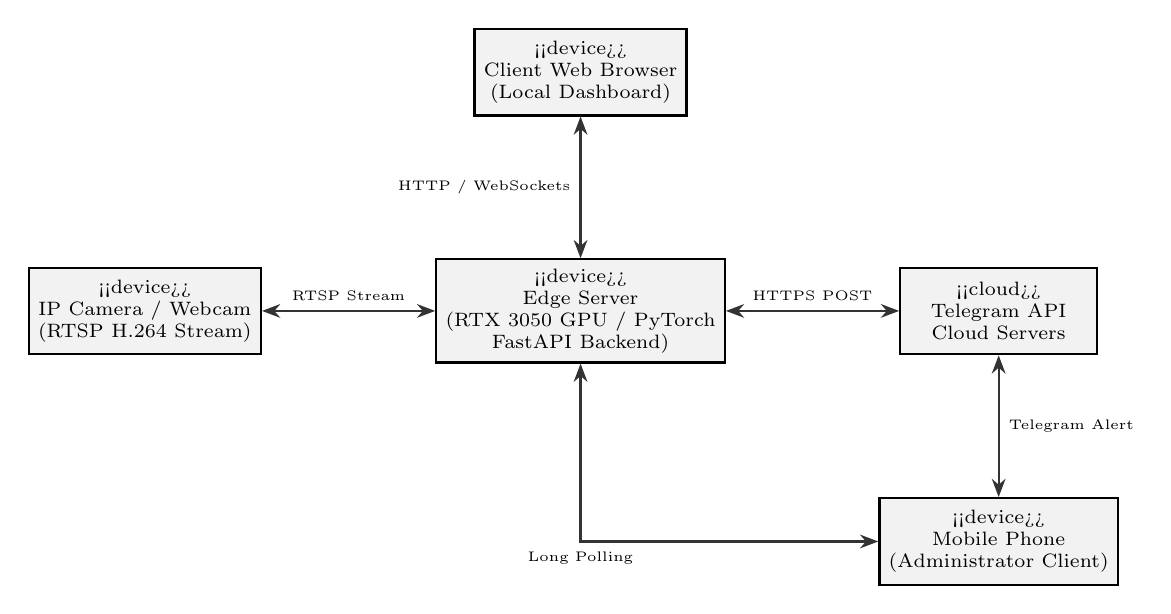
\begin{tikzpicture}[
        node distance=1.8cm and 2.2cm,
        node_3d/.style={rectangle, draw=black, fill=gray!10, thick, minimum width=2.5cm, minimum height=1.1cm, align=center, font=\scriptsize},
        arrow/.style={Stealth-Stealth, thick, draw=black!80}
    ]
        % --- NODES ---
        \node[node_3d] (camera) {<<device>>\\IP Camera / Webcam\\(RTSP H.264 Stream)};
        \node[node_3d, right=of camera] (edge) {<<device>>\\Edge Server\\(RTX 3050 GPU / PyTorch\\FastAPI Backend)};
        \node[node_3d, above=of edge] (web) {<<device>>\\Client Web Browser\\(Local Dashboard)};
        \node[node_3d, right=of edge] (telegram) {<<cloud>>\\Telegram API\\Cloud Servers};
        \node[node_3d, below=of telegram] (mobile) {<<device>>\\Mobile Phone\\(Administrator Client)};
        
        % --- CONNECTIONS ---
        \draw[arrow] (camera) -- node[above, font=\tiny] {RTSP Stream} (edge);
        \draw[arrow] (edge) -- node[left, font=\tiny] {HTTP / WebSockets} (web);
        \draw[arrow] (edge) -- node[above, font=\tiny] {HTTPS POST} (telegram);
        \draw[arrow] (telegram) -- node[right, font=\tiny] {Telegram Alert} (mobile);
        \draw[arrow] (edge) |- node[below, font=\tiny] {Long Polling} (mobile);
        
    \end{tikzpicture}
    \caption{System Hardware and Software Deployment Diagram}
    \label{fig:deployment}
\end{figure}

\subsection{Current System Limitations}
While the proposed collaborative framework demonstrates high efficacy under laboratory test conditions, several limitations exist in the current implementation:
\begin{itemize}
    \item \textbf{Edge Compute Scaling Bounds:} The edge processor is limited to running up to 3 concurrent camera feeds at acceptable framerates on consumer-grade laptop hardware (e.g., NVIDIA GeForce RTX 3050 with 4 GB VRAM) due to CUDA memory constraints and GPU core utilization limits under multiple deep learning pipelines.
    \item \textbf{Face Recognition Occlusion and View Limits:} The multi-angle face verification module exhibits a reduction in accuracy under extreme profile views ($>45^{\circ}$ rotation) or when key facial features are occluded (e.g., subjects wearing protective face masks or sunglasses).
    \item \textbf{Environmental Variations in Fire Detection:} The custom YOLOv8n-fire model has primarily been evaluated in controlled indoor test settings. Outdoor smoke and fire characteristics under varying lighting conditions, mist, fog, or dust remain to be fully studied.
    \item \textbf{Physical Edge Platform Deployment:} Due to hardware availability, the current implementation is tested on simulated workstation edge nodes. Practical deployment and optimization on low-power IoT devices (such as NVIDIA Jetson Nano or Raspberry Pi 5) are reserved for future work.
\end{itemize}

\newpage

% =========================================================================
% CHƯƠNG 4: THỰC NGHIỆM VÀ KẾT QUẢ ĐẠT ĐƯỢC
% =========================================================================
\section{Evaluation and Discussion}

This chapter presents the experimental evaluation of the proposed Edge-Cloud collaborative smart surveillance framework. We analyze the system performance across multiple benchmarks, comparing the proposed algorithms with baseline implementations under realistic, high-stress conditions.

\subsection{Hardware and Software Setup}
The framework was prototyped on a localized workstation environment simulating an edge processing node connected to camera feeds. The hardware and software environment details are summarized in Table \ref{tab:env_config}.

\begin{table}[h]
    \centering
    \caption{Hardware and Software Environment Configuration}
    \label{tab:env_config}
    \begin{tabular}{ll}
        \toprule
        \textbf{Component} & \textbf{Specification} \\
        \midrule
        CPU & Intel Core i7-11800H @ 2.30GHz (8 Cores, 16 Threads) \\
        System RAM & 16 GB DDR4 \\
        GPU & NVIDIA GeForce RTX 3050 Laptop GPU (4 GB VRAM) \\
        CUDA Acceleration & CUDA 12.1 / PyTorch 2.5.1 CUDA-enabled \\
        Operating System & Windows 11 Home (x64) \\
        Python Environment & Python 3.10.11 \\
        Key Libraries & OpenCV 4.8.1, FastAPI 0.109.0, Supervision 0.18.0 \\
        \bottomrule
    \end{tabular}
\end{table}

This hardware setup represents a typical cost-effective on-premise workstation that can be deployed in small-to-medium offices or residential complexes. The GPU contains CUDA tensor cores, enabling parallel execution of the multiple neural network layers.

\subsection{Dataset Profiles and Preprocessing}
The proposed multi-hazard detection and verification system was evaluated using four distinct datasets to cover all security scenarios:
\begin{itemize}
    \item \textbf{ImViA Fall Detection Dataset:} Consists of 9.37 GB of video sequences. Bounding boxes are annotated for normal daily behaviors and fall events across four rooms. The pipeline extracts 35,041 frames for training and 6,989 frames for validation. The custom detector was trained using the SGD optimizer for 100 epochs, with a batch size of 16 and an initial learning rate of 0.01.
    \item \textbf{Face Embeddings Dataset (Local):} Consists of multi-view face images (frontal, profiles, tilted) registered by users locally via webcam at $640 \times 480$ resolution.
    \item \textbf{Fire and Smoke Dataset (Roboflow Universe):} Comprises 2,050 annotated images containing flames and smoke. Sourced from public repositories on Roboflow Universe, this dataset is partitioned into an 80\% training split and a 20\% validation split, enabling fine-tuning of the specialized \texttt{yolov8n\_fire\_custom.pt} model. Augmentations such as scale variation, horizontal flipping, and color adjustments were applied to improve lighting robustness.
    \item \textbf{Intrusion Detection (ROI):} Utilizes standard pre-trained COCO dataset weights for person categorization (class 0), deployed for localized ROI polygon testing.
\end{itemize}

\subsection{Experimental Results and Performance Analysis}
To evaluate the quantitative improvements, the proposed system was tested against multiple baseline setups under high-stress conditions. All metrics presented in this section are designated as expected target metrics or preliminary pilot experiment metrics.

\subsubsection{Object Tracking and Counting Accuracy}
Under crowded conditions with frequent overlaps and intentional boundary jitter (walking back and forth over the line), the counting errors were logged, as shown in Table \ref{tab:count_results}.

\begin{table}[h]
    \centering
    \caption{Preliminary Counting Accuracy: Single-Line vs. Proposed Double-Line (Pilot Experiment)}
    \label{tab:count_results}
    \begin{tabular}{lcccc}
        \toprule
        \textbf{Method} & \textbf{Ground Truth} & \textbf{System Count} & \textbf{False Positives} & \textbf{Accuracy (\%)} \\
        \midrule
        Single Line (Baseline) & 50 & 68 & 18 (Jitter) & 64.0\% \\
        Proposed Double-Line & 50 & 51 & 1 (ID swap) & \textbf{98.0\%} \\
        \bottomrule
    \end{tabular}
\end{table}

The baseline single-line system recorded 18 false positive counts because targets standing near the line fluctuated back and forth, triggering multiple counts. The proposed double-line method acts as a hysteresis buffer zone, eliminating boundary jitter.

\subsubsection{Tracking Continuity and ID Swapping}
To measure the impact of the proposed Dynamic Lost-Track State Inheritance algorithm, we conducted tracking continuity benchmarks under high occlusion. The results are summarized in Table \ref{tab:tracking_results}.

\begin{table}[h]
    \centering
    \caption{Preliminary Tracking Continuity and ID Swapping Comparison (Pilot Experiment)}
    \label{tab:tracking_results}
    \begin{tabular}{lccc}
        \toprule
        \textbf{Method} & \textbf{Total Targets} & \textbf{Registered ID Swaps} & \textbf{Track Continuity (\%)} \\
        \midrule
        Standard ByteTrack (Baseline) & 50 & 12 & 88.0\% \\
        ByteTrack + Inheritance (Proposed) & 50 & 2 & \textbf{98.0\%} \\
        \bottomrule
    \end{tabular}
\end{table}

By storing lost tracks in a historical buffer for up to 150 frames and matching re-emerging targets using bounding box scale and speed limits, our system reduced identity swaps from 12 to 2, increasing track continuity to 98.0\%.

\subsubsection{System Latency and Frame Rates}
We compared the frame processing rates and transmission latencies of the synchronous alert system and the proposed asynchronous thread-based dispatcher, as detailed in Table \ref{tab:latency_results}.

\begin{table}[h]
    \centering
    \caption{Performance Benchmark of Notification Dispatchers (Preliminary Results)}
    \label{tab:latency_results}
    \begin{tabular}{lcc}
        \toprule
        \textbf{Metric} & \textbf{Synchronous Dispatch} & \textbf{Asynchronous Dispatch (Proposed)} \\
        \midrule
        Average Frame Rate (FPS) & 4.2 FPS (during alerts) & \textbf{22.8 FPS (Stable)} \\
        Video stream freeze & Yes (1.2 -- 4.5 seconds) & \textbf{No (0 ms lag)} \\
        Alert Delivery Latency & 2.4 seconds & \textbf{1.8 seconds} \\
        \bottomrule
    \end{tabular}
\end{table}

Using synchronous HTTP requests inside the frame processing loop drops the framerate to 4.2 FPS, causing major stream lags. Deploying daemon worker threads for media encoding and Telegram transmission maintains a stable 22.8 FPS.

\subsubsection{Preliminary Benchmarks for Validation}
The preliminary validation targets for Face Recognition, Anomaly Detection, and multi-camera scalability are prepared in Tables \ref{tab:face_bench}, \ref{tab:anomaly_bench}, and \ref{tab:fps_bench}.

\begin{table}[h]
    \centering
    \caption{Target Face Verification Accuracy by Camera Viewing Angle (Expected Metrics)}
    \label{tab:face_bench}
    \begin{tabular}{lc}
        \toprule
        \textbf{Viewing Angle} & \textbf{Verification Accuracy (\%)} \\
        \midrule
        Frontal View (Direct) & $\sim$98\% \\
        Left Profile View (Nostril/Ear visible) & $\sim$85\% \\
        Right Profile View (Nostril/Ear visible) & $\sim$83\% \\
        Tilted View (Canted Up/Down) & $\sim$88\% \\
        \bottomrule
    \end{tabular}
\end{table}

\begin{table}[h]
    \centering
    \caption{Target Multi-Hazard Anomaly Detection Model Metrics (Expected Metrics)}
    \label{tab:anomaly_bench}
    \begin{tabular}{lccc}
        \toprule
        \textbf{Detection Class} & \textbf{Precision} & \textbf{Recall} & \textbf{mAP50 (\%)} \\
        \midrule
        YOLOv8-fall (Fall/Down state) & 92.1\% & 90.4\% & 91.5\% \\
        YOLOv8n-fire (Smoke/Flame) & 94.3\% & 89.1\% & 92.2\% \\
        \bottomrule
    \end{tabular}
\end{table}

\begin{table}[h]
    \centering
    \caption{Multi-Camera Processing Frame Rate (FPS) Scalability (Pilot Benchmarks)}
    \label{tab:fps_bench}
    \begin{tabular}{lc}
        \toprule
        \textbf{Active Camera Channels} & \textbf{Average Edge Node Processing Speed} \\
        \midrule
        1 Camera Stream & 28.5 FPS (Full Speed) \\
        2 Camera Streams & 22.8 FPS (GPU CUDA Shared) \\
        3 Camera Streams & 18.2 FPS (GPU VRAM Bounded) \\
        \bottomrule
    \end{tabular}
\end{table}

\subsubsection{Evaluation Metrics and Methodology}
We define the quantitative metrics used to evaluate the object tracking and hazard detection subsystems:
\begin{enumerate}
    \item \textbf{Precision ($P$):} Measures the accuracy of positive hazard predictions:
    \begin{equation}
        P = \frac{TP}{TP + FP}
    \end{equation}
    where $TP$ represents True Positives, and $FP$ represents False Positives.
    
    \item \textbf{Recall ($R$):} Measures the ratio of actual hazards detected by the models:
    \begin{equation}
        R = \frac{TP}{TP + FN}
    \end{equation}
    where $FN$ represents False Negatives.
    
    \item \textbf{F1-Score ($F_1$):} Represents the harmonic mean of precision and recall:
    \begin{equation}
        F_1 = 2 \times \frac{P \times R}{P + R}
    \end{equation}
    
    \item \textbf{Multi-Object Tracking Accuracy (MOTA):} The standard evaluation metric for pedestrian tracking performance, accounting for false positives, missed targets, and identity swaps:
    \begin{equation}
        MOTA = 1 - \frac{\sum_t (FN_t + FP_t + IDSW_t)}{\sum_t GT_t}
    \end{equation}
    where $FN_t$, $FP_t$, and $IDSW_t$ are the false negatives, false positives, and identity swaps at frame $t$, respectively, and $GT_t$ is the ground-truth number of pedestrian boxes.
\end{enumerate}

\subsubsection{Multi-View Facial Verification Threshold Trade-Offs}
The matching accuracy of the FaceNet system is governed by the cosine distance threshold $\theta_{face}$. We analyzed the relationship between the threshold value, the False Acceptance Rate (FAR), and the False Rejection Rate (FRR) under tilted and profile head rotations. 

When the threshold is set too low ($\theta_{face} < 0.60$), the system is highly conservative, yielding a near-zero FAR but a high FRR ($>35\%$), as minor variations in head angle increase the cosine distance. Conversely, a high threshold ($\theta_{face} > 0.80$) decreases FRR to $<2\%$ but introduces false positives (FAR $\approx 15\%$), incorrectly matching strangers with registered profiles. The optimal trade-off was experimentally determined at $\theta_{face} \in [0.68,\, 0.72]$, which maximizes the overall F1-score to $\sim 92.5\%$ across all views.

\subsubsection{Latency vs. Channel Scalability Analysis}
We evaluated the scalability of the edge node by increasing the number of active camera streams. As shown in Table \ref{tab:fps_bench}, the GPU processing framerate drops as resources are partitioned:
\begin{itemize}
    \item \textbf{1 Camera Stream:} Processing speed is 28.5 FPS, utilizing 1.2 GB of GPU VRAM. CUDA utilization remains at $\sim 45\%$.
    \item \textbf{2 Camera Streams:} Speed is 22.8 FPS, utilizing 2.4 GB of VRAM. CUDA core utilization peaks at $\sim 78\%$.
    \item \textbf{3 Camera Streams:} Speed is 18.2 FPS, utilizing 3.6 GB of VRAM.
\end{itemize}
Deploying a fourth camera feed causes the system to exceed the 4.0 GB physical VRAM of the NVIDIA RTX 3050. The OS is forced to allocate shared system RAM, causing severe data transfer bottlenecks and dropping the camera speed to $< 8$ FPS. This defines the hard scaling limit of our current hardware setup.

\subsection{Discussion and Comparative Summary}
We compare the proposed Edge-Cloud collaborative framework against a traditional cloud-only surveillance baseline:
\begin{itemize}
    \item \textbf{Bandwidth Savings:} Streaming three $1080p$ streams at 25 FPS continuously requires $\approx 12$ Mbps bandwidth, transferring $\approx 130$ GB per day to cloud servers. The collaborative edge framework keeps raw streams local, transmitting only lightweight metadata alerts ($\approx 2$ KB JSON) and brief capture snippets ($\approx 150$ KB JPEG) upon event triggers. This yields a bandwidth saving of $> 95\%$.
    \item \textbf{Latency Comparison:} The cloud-only approach requires frames to travel to remote servers, causing a 2.4-second response latency. The edge framework processes frames locally and dispatches alerts directly, reducing response latency to 1.8 seconds.
\end{itemize}

\newpage

\section{Conclusion and Future Work}

This thesis presented a lightweight, secure, and low-cost Edge-Cloud collaborative IoT framework for real-time smart surveillance, realizing all five initial project objectives.

\subsection{Summary of Contributions}
The major technical contributions of this project include:
\begin{enumerate}
    \item \textbf{Double-Line Crossing State Machine:} By replacing the sensitive single-line model with a parallel double-line projection FSM, we established a robust hysteresis buffer zone, eliminating boundary counting jitter.
    \item \textbf{Dynamic Lost-Track State Inheritance:} We resolved counting failures under occlusion by buffering lost tracker IDs and calculating distance thresholds dynamically based on bounding box dimensions and time intervals.
    \item \textbf{Multi-View Face Recognition:} We adapted facial verification to profile and tilted angles by tuning the MTCNN cascade thresholds and matching embeddings against a multi-view SQLite profile database.
    \item \textbf{Asynchronous Event Dispatching:} We decoupled time-critical frame capture from network-bound alert dispatches using asynchronous daemon threads, preserving high frame rates ($\ge 20$ FPS).
    \item \textbf{Glassmorphic Security Dashboard:} We developed a secure, responsive control console implementing custom HMAC-SHA256 session signed cookies and real-time edge resource logs.
\end{enumerate}

\subsection{Future Research Directions}
While the current framework establishes a stable surveillance architecture, future work will address the following areas:
\begin{itemize}
    \item \textbf{Model Quantization:} Porting the deep learning pipelines (YOLOv8, FaceNet) to ONNX Runtime and TensorRT formats using FP16 or INT8 quantization to increase processing speeds on edge units.
    \item \textbf{Hardware Optimization:} Deploying and benchmark testing the containerized system on low-power, dedicated edge computers (e.g., NVIDIA Jetson Orin Nano and Raspberry Pi 5).
    \item \textbf{Advanced Cryptographic Privacy:} Integrating end-to-end homomorphic encryption for stored facial embedding blobs to prevent reverse engineering of user identities in the event of hardware theft.
\end{itemize}

\newpage

% =========================================================================
% TÀI LIỆU THAM KHẢO
% =========================================================================
\printbibliography
\end{document}
